%%%%%%%%%%%%
%
% $Autor: Wings $
% $Datum: 2019-03-05 08:03:15Z $
% $Pfad: Sketch.tex $
% $Version: 4250 $
% !TeX spellcheck = en_GB/de_DE
% !TeX encoding = utf8
% !TeX root = manual 
% !TeX TXS-program:bibliography = txs:///biber
%
%%%%%%%%%%%%

\section*{User Interface Sketch}

The figure below provides a schematic overview of the main elements in the user interface of the Hurricane Intensity Prediction App. This helps users understand what to expect when running the application.

\begin{figure}[h]
	\centering
	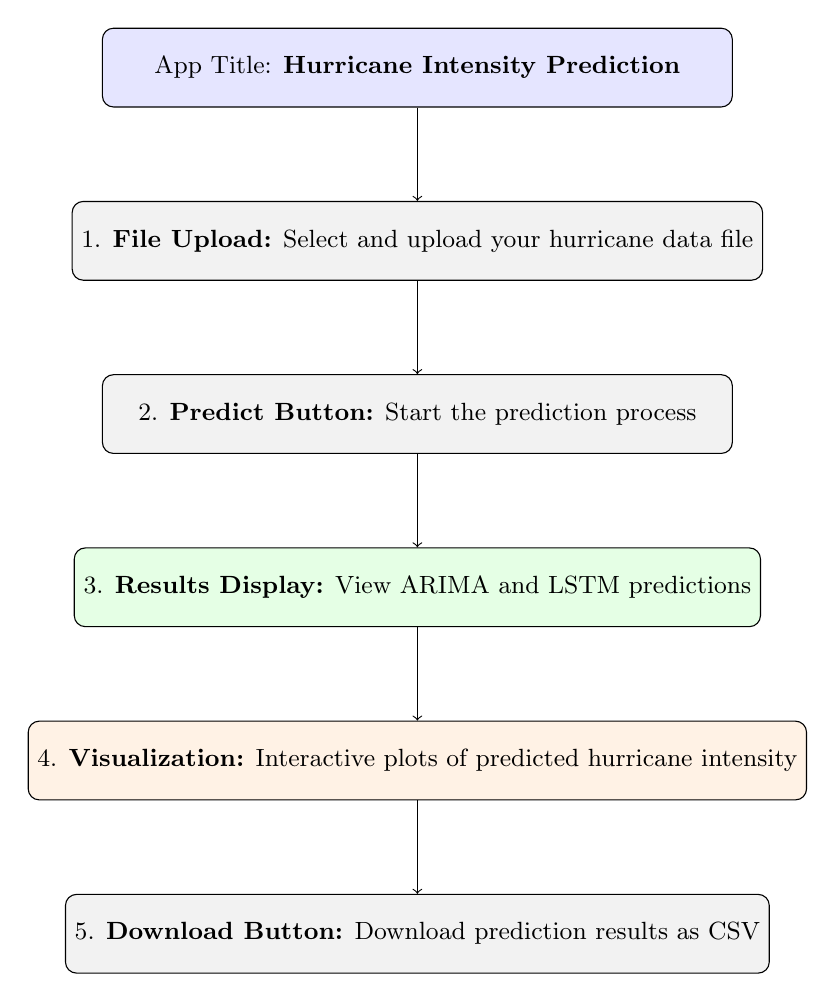
\begin{tikzpicture}[
		node distance=2.2cm, % Increased vertical space between nodes
		every node/.style={draw, rounded corners, minimum width=8cm, minimum height=1cm, align=left, font=\small}
		]
		% App title
		\node[fill=blue!10] (title) {App Title: \textbf{Hurricane Intensity Prediction}};
		% File upload
		\node[below of=title, fill=gray!10] (upload) {1. \textbf{File Upload:} Select and upload your hurricane data file};
		% Predict button
		\node[below of=upload, fill=gray!10] (predict) {2. \textbf{Predict Button:} Start the prediction process};
		% Results display
		\node[below of=predict, fill=green!10] (results) {3. \textbf{Results Display:} View ARIMA and LSTM predictions};
		% Visualization
		\node[below of=results, fill=orange!10] (visual) {4. \textbf{Visualization:} Interactive plots of predicted hurricane intensity};
		% Download button
		\node[below of=visual, fill=gray!10] (download) {5. \textbf{Download Button:} Download prediction results as CSV};
		
		% Arrows
		\draw[->] (title) -- (upload);
		\draw[->] (upload) -- (predict);
		\draw[->] (predict) -- (results);
		\draw[->] (results) -- (visual);
		\draw[->] (visual) -- (download);
	\end{tikzpicture}
	\caption{Sketch of the User Interface for the Hurricane Intensity Prediction App}
\end{figure}
